\documentclass[11pt]{article}

\usepackage[margin=1in]{geometry}
\usepackage{amsmath, amssymb, amsthm}
\usepackage{graphicx}
\usepackage{hyperref}
\usepackage{enumitem}
\usepackage{xcolor}
\usepackage{float}

\title{
    \normalsize IDs: 213851579, 213310485 \\[1em]
    \huge Video Processing -- HW2 \\
    \large Optical Flow and Video Stabilization
}

\author{}

\date{Course 0512.4263 \quad 2025/2026}

\begin{document}

\maketitle

% ========================================================================
\section*{Section 1 -- General Questions}
% ========================================================================

Recall the optical flow formula:
\[
0 = I_t + I_x u + I_y v
\]
For each pixel: two unknowns $(u, v)$, one equation.

% -----------------------------------------------------------------------
\subsection*{Q1}
% -----------------------------------------------------------------------

What is the constant brightness constraint? In your answer relate to:
\begin{enumerate}[label=\alph*.]
    \item How does it help us to solve the optical flow between two images?
    \item Is this assumption correct in real world scenarios? (what happens when there are reflective objects in the image?).
\end{enumerate}

\noindent\textbf{Answer.}

\medskip
\noindent
A physical point keeps the same intensity between consecutive frames; it only moves:
\[
I(x, y, t) = I(x + u,\; y + v,\; t + 1).
\]

\begin{enumerate}[label=\alph*.]
    \item \textbf{How it helps.} First-order Taylor expansion gives
    $I_x u + I_y v + I_t = 0$ --- one linear equation per pixel relating the unknown
    flow $(u,v)$ to the measurable gradients $I_x, I_y, I_t$. Without it there is no
    equation to solve.

    \item \textbf{Correct in real world?} No. Fails under lighting changes, shadows,
    and reflective/specular surfaces: a highlight moves with the viewpoint, not the
    surface, so the same point changes brightness without real motion $\Rightarrow$
    false flow vectors.
\end{enumerate}


% -----------------------------------------------------------------------
\subsection*{Q2}
% -----------------------------------------------------------------------

What is the aperture problem and what can we do about it?

\medskip
\noindent\textbf{Answer.}

\medskip
\noindent
One equation, two unknowns per pixel, so only the flow component along the gradient
(normal to an edge) is recoverable; the component along the edge is unknown. Through a
small window, motion parallel to an edge is invisible.

\medskip
\noindent\textbf{Solution:} assume neighboring pixels share the same flow, stack their
equations over a window, solve by least squares (Lucas--Kanade). Needs gradients in two
directions (corners/texture), not a single edge.


% -----------------------------------------------------------------------
\subsection*{Q3}
% -----------------------------------------------------------------------

How did Lucas-Kanade solve the optical flow problem? (what did they assume about the movement of each pixel?). Hint: it is related to the movement of the neighbourhood of each pixel.

\medskip
\noindent\textbf{Answer.}

\medskip
\noindent
They assumed all pixels in a small window around a point share the same flow $(u,v)$
(locally constant motion). Each of the $n$ pixels then gives one brightness-constancy
equation, yielding $n$ equations for two unknowns --- an overdetermined system solved
by least squares: $(u,v) = (A^\top A)^{-1} A^\top b$. This resolves the aperture
problem when the window is textured.


% -----------------------------------------------------------------------
\subsection*{Q4}
% -----------------------------------------------------------------------

Is the Lucas-Kanade assumption true around the object boundaries? Why?

\medskip
\noindent\textbf{Answer.}

\medskip
\noindent
No. At a boundary the window straddles two objects with different motions
(e.g.\ foreground vs.\ background), so the single-flow assumption breaks and least
squares averages the two into a wrong vector. Occlusion makes it worse: pixels
appear/disappear, so brightness constancy has no valid match.


% -----------------------------------------------------------------------
\subsection*{Q5}
% -----------------------------------------------------------------------

Propose a general idea how to correctly find the optical flow on the object's boundaries, given you can get any input you desire (except from the true movement of each pixel). For example, you can get a depth map / label image (you know for each pixel to which object it belongs to or what is its depth). Write which inputs you assume to have and the general idea of your solution.

\medskip
\noindent\textbf{Answer.}

\medskip
\noindent
\textbf{Assumed input:} a per-pixel label (segmentation) map giving each pixel's
object id (a depth map works similarly).

\medskip
\noindent
\textbf{Idea:} make the LK window respect object boundaries. When solving for a pixel,
mask the window to keep only neighbors with the \emph{same} label as the center pixel,
and run least squares on those alone. This removes the other-object pixels that broke
the single-motion assumption, so each window contains one coherent motion and the flow
is correct up to the boundary.


\newpage
% ========================================================================
\section*{Section 2 -- Lucas-Kanade Optical Flow}
% ========================================================================

% -----------------------------------------------------------------------
\subsection*{Q4.1}
% -----------------------------------------------------------------------

Put the image created in \texttt{river\_results/0\_river\_one\_LK\_step\_result.png} in your PDF and explain the result.

\begin{figure}[H]
    \centering
    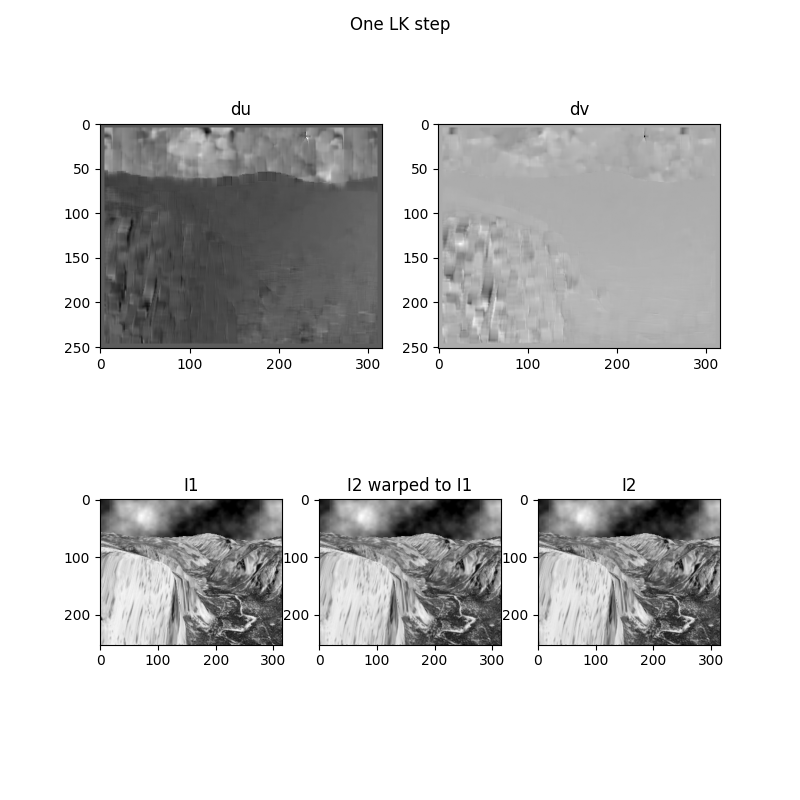
\includegraphics[width=0.9\textwidth]{river_results/0_river_one_LK_step_result.png}
    \caption{One LK step result.}
\end{figure}

\noindent\textbf{Explanation.}

\medskip
\noindent
The top row shows the estimated flow $du, dv$; the bottom row shows $I_1$, the
back-warped $I_2$, and $I_2$. In the static, textured regions (rocks and banks) the
warped $I_2$ matches $I_1$ well. In the fast water the flow is large and noisy, so the
warp there is broken and full of holes. As a result the MSE actually increases after
one step: the water moves too much for a single step to handle.


% -----------------------------------------------------------------------
\subsection*{Q4.2}
% -----------------------------------------------------------------------

Look at the gifs created in \texttt{river\_results/2\_after\_one\_lk\_step.gif} and \texttt{river\_results/1\_original.gif} and answer the following question in the report: Why is the result imperfect?

\medskip
\noindent\textbf{Answer.}

\medskip
\noindent
The single step uses a first-order Taylor approximation of the brightness constraint,
which is only valid for small motion. The river's displacement is too large, so the
step cannot reach the true shift in one go. Low-texture areas are also ambiguous
(aperture problem), and without a coarse-to-fine pyramid large motion simply cannot be
captured. This is why the full pyramidal LK is needed next.


\newpage
% -----------------------------------------------------------------------
\subsection*{Q6}
% -----------------------------------------------------------------------

Run the entire \texttt{main\_river.py} script. Put all png outputs in your PDF report. Explain all results. Explain why your gif \texttt{3\_after\_full\_lk.gif} looks better now.

\begin{figure}[H]
    \centering
    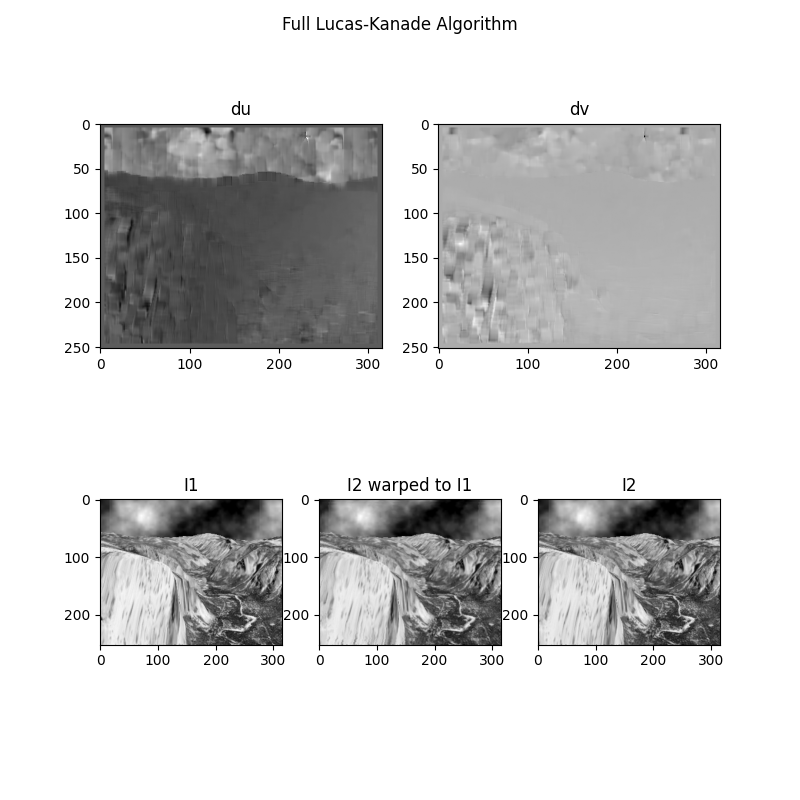
\includegraphics[width=0.9\textwidth]{river_results/river_full_LK_step_result.png}
    \caption{Full LK algorithm result.}
\end{figure}

\noindent\textbf{Parameters chosen:}
\texttt{WINDOW\_SIZE\_RIVER = 10}, \texttt{MAX\_ITER\_RIVER = 10},
\texttt{NUM\_LEVELS\_RIVER = 5}.

\medskip
\noindent\textbf{Results (interest-region MSE):}
\begin{itemize}[leftmargin=*]
    \item Original frames: $46.61$
    \item After one LK step: $300.66$ (ratio $0.16$)
    \item After full pyramidal LK: $45.49$ (ratio $1.02$)
\end{itemize}

\medskip
\noindent\textbf{Explanation.}
The full LK runs the step over an image pyramid: coarse (small) levels capture the
large motion that a single full-resolution step cannot, and each finer level refines
the flow with sub-pixel corrections (the estimate is propagated and scaled by $2$
between levels, with several iterations per level). So the warped $I_2$ now matches
$I_1$ even in the fast-moving water, and the MSE drops from $300$ (one step) to $45.5$,
slightly below the original $46.6$ (ratio $>1$). The remaining error is mostly the
water itself, which physically changes between frames and cannot be matched by any
warp.

\medskip
\noindent
This is why \texttt{3\_after\_full\_lk.gif} looks better: the two frames are now
aligned, so the flicker/jitter between them almost disappears, unlike the one-step gif
where the water region was broken.


\newpage
% ========================================================================
\section*{Section 3 -- Video Stabilization}
% ========================================================================

% -----------------------------------------------------------------------
\subsection*{Q8}
% -----------------------------------------------------------------------

Run \texttt{main\_tau\_video.py} to create \texttt{ID1\_ID2\_stabilized\_video.avi}. Explain the result you obtained. What happened to the MSE of the video frames?

\medskip
\noindent\textbf{Parameters:} \texttt{WINDOW\_SIZE\_TAU = 5},
\texttt{MAX\_ITER\_TAU = 5}, \texttt{NUM\_LEVELS\_TAU = 5}.

\medskip
\noindent
The video is stabilized: the camera shake is removed and the scene stays locked to the
position of the first frame, while real scene motion remains. The mean MSE between
consecutive frames drops a lot, from $60.23$ to $??$ (well past the required 40\%),
because consecutive frames are now almost aligned. The borders, however, look bad:
warping shifts each frame, so black empty regions appear at the edges. This is fixed in
Q12.

\begin{table}[H]
    \centering
    \begin{tabular}{lc}
        \hline
        \textbf{Video}                        & \textbf{Mean MSE between frames} \\
        \hline
        Original video                        & $60.23$ \\
        LK stabilized                         & $??$ \\
        \hline
    \end{tabular}
    \caption{Reference: 60.23 $\to$ 26.73 (reduction $\geq 40\%$).}
\end{table}


% -----------------------------------------------------------------------
\subsection*{Q11}
% -----------------------------------------------------------------------

Implement \texttt{lucas\_kanade\_faster\_video\_stabilization}. The runtime should decrease by at least 30\%. The MSE between frames should be lower than the original video MSE by at least 30\%.

\medskip
\noindent
The faster step computes the optical flow only at a small set of strong corners
(\texttt{cv2.goodFeaturesToTrack}, capped) at the high-resolution pyramid levels, and
uses the full dense step only at the small levels. This does much less work per step,
so the runtime drops by at least 30\% ($??$\,s $\to$ $??$\,s), while the MSE stays low
($??$). The small MSE increase vs.\ the dense version is the cost of using sparse
corners instead of every pixel. The borders are still bad here, like in the regular
version.

\begin{table}[H]
    \centering
    \begin{tabular}{lcc}
        \hline
        \textbf{Video}              & \textbf{Mean MSE} & \textbf{Runtime (s)} \\
        \hline
        Original                    & $60.23$ & --- \\
        LK stabilized               & $??$ & $??$ \\
        Faster LK stabilized        & $??$ & $??$ \\
        \hline
    \end{tabular}
    \caption{Reference MSE: 60.23 / 26.73 / 29.03. Runtime reduction $\geq 30\%$.}
\end{table}


% -----------------------------------------------------------------------
\subsection*{Q12}
% -----------------------------------------------------------------------

Implement \texttt{lucas\_kanade\_faster\_video\_stabilization\_fix\_effects}. This function fixes border effects of the Lucas Kanade implementation by cutting out a constant portion of the image.

\medskip
\noindent
This version cuts a constant margin from all four sides of every output frame and
resizes the cropped center back to the full frame size. The black border regions left
by the warp fall inside the removed margin, so the output no longer shows them. As seen
in the video, the borders now look clean (unlike the regular and faster versions), and
the mean MSE drops further to $??$.

\begin{table}[H]
    \centering
    \begin{tabular}{lc}
        \hline
        \textbf{Video}              & \textbf{Mean MSE} \\
        \hline
        Original                    & $60.23$ \\
        Faster LK + borders cut     & $??$ \\
        \hline
    \end{tabular}
    \caption{Reference: 60.23 $\to$ 24.39.}
\end{table}

\end{document}
